% Name: Cloud with rain
% Description: A gray cloud with teardrop raindrops falling from it.
% Tags: cloud, rain, weather, illustration

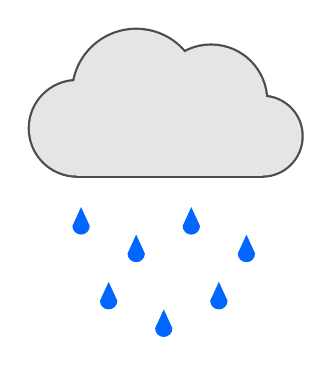
\begin{tikzpicture}
  % Outline every circle first, then fill them all, so only the outer edge of the cloud is drawn
  \foreach \p/\r in {{(-1.1,0)/0.6}, {(-0.35,0.45)/0.8}, {(0.6,0.35)/0.7}, {(1.25,-0.1)/0.5}}
    \draw[gray!60!black, line width=1.6pt] \p circle (\r);
  \draw[gray!60!black, line width=1.6pt] (-1.1,-0.6) rectangle (1.25,0);
  \foreach \p/\r in {{(-1.1,0)/0.6}, {(-0.35,0.45)/0.8}, {(0.6,0.35)/0.7}, {(1.25,-0.1)/0.5}}
    \fill[gray!20] \p circle (\r);
  \fill[gray!20] (-1.1,-0.6) rectangle (1.25,0);
  % Raindrops: a point on top, a half circle below
  \foreach \x/\y in {-1.05/-1.0, -0.35/-1.35, 0.35/-1.0, 1.05/-1.35, -0.7/-1.95, 0.7/-1.95, 0/-2.3} {
    \fill[blue!60!cyan] (\x,\y) -- ++(-0.11,-0.24) arc[start angle=180, end angle=360, radius=0.11] -- cycle;
  }
\end{tikzpicture}
